The logistic model was applied to both the Kiddivax and the Ha Nam data.

The resulting protection curve for Kiddivax is in Figure \ref{fig:kiddyvaxmain-prot-lr} and for Ha Nam --- in Figure \ref{fig:hanam-prot-lr}. The resulting relative-to-5 protection curve for Kiddivax is in Figure \ref{fig:kiddyvaxmain-prot-rel-lr-boot} and for Ha Nam --- in Figure \ref{fig:hanam-prot-rel-lr-boot}.

\begin{figure}[htp]
    \centering
    \includegraphics[width=0.5\textwidth]{../preds-plot/kiddyvaxmain-lr-bvic.pdf}
    \caption{
        Fitted protection curves and confidence intervals from the standard logistic model fit to Kiddivax data. The solid line is the point estimates. The shaded region is the 95\% confidence interval.
    }
    \label{fig:kiddyvaxmain-prot-lr}
\end{figure}

\begin{figure}[htp]
    \centering
    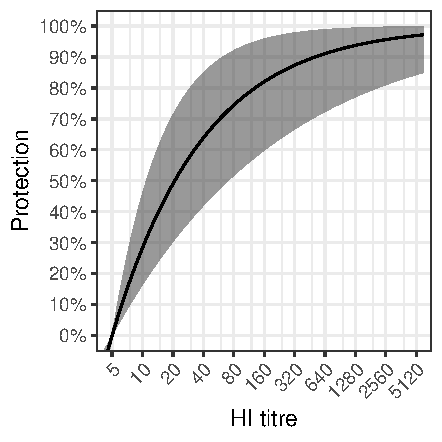
\includegraphics[width=0.5\textwidth]{../fit-logistic-boot-plot/kiddyvaxmain-bvic-prot-rel.pdf}
    \caption{
        Fitted relative-to-5 protection curves and confidence intervals from the standard logistic model fit to the B Victoria subset of Kiddivax data. The solid line is the point estimates. The shaded region is the 95\% confidence interval. The bounds for the confidence interval were obtained by using the bootstrap method (10,000 samples).
    }
    \label{fig:kiddyvaxmain-prot-rel-lr-boot}
\end{figure}

\begin{figure}[htp]
    \centering
    \includegraphics[width=0.8\textwidth]{../preds-plot/hanam-hi-lr-h3.pdf}
    \caption{
        Fitted protection curves and confidence intervals from the standard logistic model fit to Ha Nam data. The solid line is the point estimates. The shaded region is the 95\% confidence interval.
    }
    \label{fig:hanam-prot-lr}
\end{figure}

\begin{figure}[htp]
    \centering
    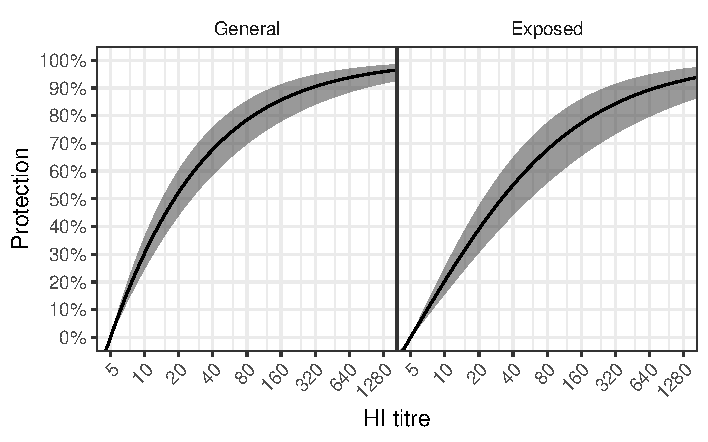
\includegraphics[width=0.8\textwidth]{../fit-logistic-boot-plot/hanam-h3-prot-rel.pdf}
    \caption{
        Fitted relative-to-5 protection curves and confidence intervals from the standard logistic model fit to the H3N2 subset of the Ha Nam data. The solid lines are the point estimate. The shaded region is the 95\% confidence interval. The bounds for the confidence interval were obtained by using the bootstrap method (10,000 samples).
    }
    \label{fig:hanam-prot-rel-lr-boot}
\end{figure}

While the relative-to-5 protection curves appear more plausible than the relative-to-baseline protection curves, both result from fitting a model with an unsatisfied assumption (baseline of 1) and neither method of generating protection curves from logistic regression model reliably produces accurate results. In addition, the high confidence in the results is misplaced as it is a result of a string assumption on the data that is unfounded.

The relative-to-5 curves present an additional problem. The curve shows how much ``better'' different titres are at protecting against infection than the titre of 5.
There is nothing inherently special about this threshold of 5. Its choice is based on the lower dilution of 10 which is necessitated by the pre-treatment of sera. The curves may look substantially different if a different threshold (e.g. 10 or 1) is chosen. This hampers the interpretability and comparison of results.
